\documentclass{article}
\newcommand\hmmax{0}
\newcommand\bmmax{0}
\usepackage{booktabs}

%% Language and font encodings
\usepackage[english]{babel}
\usepackage[utf8x]{inputenc}
\usepackage[T1]{fontenc}
\usepackage{gensymb}
\usepackage{pdfpages}
\usepackage{mparhack}


\usepackage[bitstream-charter]{mathdesign}
\let\circledS\undefined
%% Sets page size and margins
\usepackage[a4paper,top=2cm,bottom=2cm,left=1cm,right=7cm,marginparwidth=5cm, marginparsep=1cm]{geometry}

\newtheorem{theorem}{Theorem}[section]
\newtheorem{corollary}{Corollary}[theorem]
\newtheorem{lemma}[theorem]{Lemma}
\newtheorem{definition}{Definition}[section]
\newtheorem{principle}{Principle}[section]

%% Useful packages
\usepackage{amsmath}
\usepackage{bm}
\usepackage{enumitem}
\usepackage{listings}
\usepackage{multirow}
\usepackage{amssymb}
\usepackage{float}
\usepackage{graphicx}
\usepackage[]{appendix}
\usepackage{wrapfig}

\usepackage[noend]{algpseudocode}
\usepackage{algorithm,algorithmicx}


\newcommand*\Let[2]{\State #1 $\gets$ #2}
\algrenewcommand\algorithmicrequire{}
\algrenewcommand\algorithmicensure{\textbf{Postcondition:}}


\newcommand{\ix}[1]{%
  \leavevmode % if at the start of a paragraph
  \marginpar{\small\emph{#1}}% the note
}

\newcommand{\comment}[1]{
	\textcolor{red}{\textbf{#1}}
}

\DeclareMathAlphabet{\altmathcal}{OMS}{cmsy}{m}{n}

\title{\textbf{Reinforcement Learning: An Introduction}\\
\textit{Summary Notes}
}
\author{Mrinank Sharma}

\begin{document}
\maketitle

\section{Introduction}
Other\ix{Elements of Reinforcement Learning} than the \textbf{agent} and the \textbf{environment}, there are four main subelements of an RL system:
\begin{enumerate}
	\item The \emph{policy} maps perceived states of the environment to actions. This could be a lookup table or a search process. 
	\item The \emph{reward signal} defines the goal of a reinforement learning problem. The environment sends rewards to an agent that has the sole objective of maximising this reward. 
	\item The \emph{value function} specifies what is good in the long run. The \emph{value} of a state is the total amount of reward an agent can expect to accumulate over teh future starting from that state. 
	\item Some RL systems have \emph{models} of the environment that can mimic the behaviour of the environment. Models are used for planning. 
\end{enumerate}
Whilst\ix{Rewards and Value Functions} rewards determine the immediate, intrisic desirability of environmental states, values indicate  the long-term desirability of states after taking into account which states are likely to follow. We choose actions based on values, even though values are derived from rewards.  

It\ix{Evolutionary Methods} is possible to learn policies without estimating value functions by using evolutionary methods. However, they tend to ignore much of the useful structure and are not well suited for RL tasks as they ignore relevant information, such as the states which are passed and the actions which are selected. 

\section{Multi-armed Bandits}
\begin{quote}
	\emph{The most important feature distinguishing reinforcement learning from other types of learning is that it uses training information that \textbf{evaluates} the actions taken rather than \textbf{instructs} by giving correct actions.}
\end{quote}
This form of feedback creates the need for active exploration. 

\begin{definition}[$k$-armed Bandit]
	\ix{$k$-armed bandits}In the $k$-armed bandit problem, you are repeatedly faced with a choice among $k$ different actions. After each choice, a numerical reward is received from a \textbf{stationary} probability distribution associated with the selected action. The objective is to maximise the expected total reward over some time period. 
\end{definition}
The \ix{Value}value of action $a$ is the expected reward given $a$ was chosen:
\begin{align}
q_*(a) = \mathbb{E}[R_t |\ A_t = a].
\end{align}
If we knew the values, problem solved - just pick the action with the maximum value. However, we do not know these. Denote the \emph{estimated} value as $Q_t(a)$. A simple way to estimate the action-value is a \emph{sample average}, which can be calculated incrementally. 

Note\ix{Reward Variance} that purely greedy methods are best if there is no noise in the reward signal. With $\epsilon$-greedy algorithms, the best value of $\epsilon$ will depend on the amount of noise, which determines the number of samples for the sample average to converge. However, if the problem is \emph{non-stationary}, we still need to explore.  

If\ix{Non-stationary Problems} the bandit is non-stationary, we might use the following rule for value estimates:
\begin{align}
Q_{n+1}(a) = Q_{n}(a) + \alpha_n(a)\ \big[ R_n - Q_n(a)\big].
\end{align}
It\ix{Convergence Guarantees} is known that convergence with probability $1$ happens if the following conditions hold:
\begin{align}
	\sum_{n=1}^{\infty} \alpha_n(a) = \infty \text{,  and } \sum_{n=1}^{\infty} \alpha_n(a)^2 < \infty.
\end{align}
The first condition ensures the steps are sufficiently large to overcome an initial condition and the second condition ensures that the steps become small enough to give convergence. However, step sizes which meet this conditions are rarely used in applications because they seem to converge slowly or require considerable tuning. 

With this techniques, the initialisation effectively becomes an additional parameter which needs to be chosen. They can be used to provide prior knowledge and can encourage exploration, for example, by being optimistic. However, this sort of exploration is not useful for non-stationary problems (the task changes creates a renewed need for exploration). 

The\ix{UCB} intuition behind UCB is that its better, when exploring, to select among the non-greedy actions which have the \emph{potential} for being optimal. To do this, we maximise an estimate of the arm's value summed with some sort of uncertainty estimate. UCB often performs well but can be difficult to extent to RL from bandits. 

We don't have to use value based methods. Instead, we could directly learn a preference over the actions and modify our preferences to give us higher rewards e.g., increasing our preference for an action if selecting it lead to a better outcome than expected. 

\begin{definition}[Contextual Bandits]
	In\ix{Contextual Bandits} a contextual bandit, the agent is faced with a series of multi-armed bandit problems, each associated with some information i.e., the agent has information about which bandit problem is being faced at any timestep. 
\end{definition}
Contextual bandits are intermediate between multi-armed bandits and the full RL problem; they involve learning a policy (i.e., a mapping from state information to actions) but similar to $k$-armed bandits, \textbf{the action selected influences only the immediate reward and not the next situation}. If we drop this constraint, we have the full RL problem. 

\section{Finite Markov Decision Processes}
\begin{definition}[Finite Markov Decision Process (MDP)]
	A\ix{MDP} finite Markov Decision Process (MDP) is made up of:
	\begin{itemize}[noitemsep]
		\item A sequence of discrete time steps, $t = 0, 1, 2, \ldots$.
		\item A discrete set of states, $S_t \in \altmathcal{S}$.
		\item A set of actions which the agent can take, $A_t \in \altmathcal{A}(S_t)$.
		\item A finite set of numerical rewards, $R_t \in \altmathcal{R} \subset \mathbb{R}$.
	In this case, there is a well defined discrete transition distribution:
	\begin{align}
	p(s', r | s, a) \triangleq \text{Pr}[S_t = s', R_t =r| S_{t-1}=s, A_{t-1}=a],
	\end{align}
	which defines the \textbf{dynamics} of the MDP. 
	\end{itemize}
\end{definition}
Note the Markov assumption; probabilities over the next state and reward depend only on the current state and action.\ix{Interpreting the Markov Assumption} This can be interpreted as a restriction on the state - the state must include information about all aspects of the past agent-environment interaction which will affect the future. 

Given $p$, we can compute the following functions of interest:
\begin{align}
p(s'|s, a) \triangleq \text{Pr}[S_t = s' | S_{t-1}=s, A_{t-1}=a],
\end{align}
\begin{align}
r(s, a) \triangleq \mathbb{E}[R_t  | S_{t-1}=s, A_{t-1}=a],
\end{align}
and
\begin{align}
r(s, a, s') \triangleq \mathbb{E}[R_t  | S_{t-1}=s, A_{t-1}=a, S_t = s'].
\end{align}

A\ix{Agent vs Environment} general rule of thumb is that anything that cannot be changed \emph{arbitarily} by the agent is considered to be outside of it and thus part of the environment. The agent-environment boundary represents the limit of the agent's absolute control, not of its knowledge. 

The goal of the agent is formalised in terms of the reward signal which passes from the environment to the agent. This is one of the most distinctive features of RL. 
\begin{quote}
	\ix{Reward Hypothesis}\emph{All of what we mean by goals and purposes can be well though of as the maximisation of the expected value of the cumulative sum of a received scalar signal.}
\end{quote}
The reward signal is not the place to impart to the agent prior knowlege about \emph{how} to achieve a task; if we do this, the agent may only achieve subgoals without actually acheiving the real goal. A better place to impart this knowledge is the initial policy or value function. \comment{How does this link to reward shaping?}

\ix{Discount Rates}Episodic tasks terminate at some timestep, $T$, whilst continuing tasks do not. In the first case, we simply use the (expected) sum of rewards whilst we introduce discounting in the infinite horizon case i.e., 
\begin{align}
G_t \triangleq \sum_{k=0}^{\infty} \gamma^k R_{t+k+1}.
\end{align}
$G_t$ is the \emph{discounted return}. The closer the value of $\gamma$ is to $1$, the more farsighted the agent is. 

\ix{Unifying Notation}We convert episodic tasks to continuing tasks by introducting a special \emph{absorbing state} which transitions only to itself and returning zero reward. We can write:
\begin{align}
G_t \triangleq \sum_{k=t+1}^{T} \gamma^{k-t-1} R_k,
\end{align}
allowing for $T=\infty$ and $\gamma=1$. \comment{The book says not both - but I think that should be allowed for an episodic task with absorbing state.}

\begin{definition}[Policy]
	\ix{Policy}A policy is a mapping from states to probabilities of selecting each possible action. $\pi(a|s)$ is the distribution over actions, $A_t$, given the current state, $S_t$. 
\end{definition}

\begin{definition}[Value Function]
	The\ix{Value Function} value function of state $s$ under policy $\pi$ is the expected return when starting in $s$ and following $\pi$.
	\begin{align}
	v_\pi(s) \triangleq \mathbb{E}_\pi [G_t | S_t = s]
	\end{align}
\end{definition}

\begin{definition}[Action-Value Function]
	The\ix{Action-Value Function} action-value function of action $a$, state $s$ under policy $\pi$ is the expected return when starting in $s$ and following $\pi$ after first performing $a$.
	\begin{align}
	q_\pi(s, a) \triangleq \mathbb{E}_\pi [G_t | S_t = s, A_t = a]
	\end{align}
\end{definition}
Value functions satisfy recursive relationships. 

A\ix{Optimal Policies} policy, $\pi$, is better than policy $\pi'$ iff $v_\pi(s) \geq v_{\pi'}(s) \forall s \in \altmathcal{S}$ with a strict inequality for at least one state. Optimal policies are better than or equal to all other policies. There may be multiple optimal policies, but they all share the same state-value function, 
\begin{align}
v_*(s) = \max_\pi v_\pi(s), \text{ for all } s \in \altmathcal{S}. 
\end{align}
The optimal action-value function is define analogously. 

\ix{Bellman Optimality Equality}The Bellman optimality equation for the value function is:
\begin{align}
v_*(s) = \max_{a \in \altmathcal{A}(s)} \sum_{s' \in \altmathcal{S}, r \in \altmathcal{R}} p(s', r | s, a) [r + \gamma v_*(s')],
\end{align}
which expresses the intuition that the optimal value of a state is equal to the expected return of the best action from that state. Similarly, for the action-value function, 
\begin{align}
q_*(s, a) = \sum_{s', r} p(s', r | s, a) [r + \gamma \max_{a' \in \altmathcal{A}(s')} q_*(s', a')].
\end{align}
For a finite MDP, the Bellman optimality equations give a system of equations which can be solved for $v_*(s)$. Once we have the optimal value functions, it is easy to determine an optimal policy by acting greedily (or performing a one-step search).  \textbf{If you use $v_*$ to select actions in the short-term, the greedy policy is optimal in the long term since this value function takes into account reward consequences.} The optimal expected long-term return is locally and immediately available for each state so a one-step lookahead search yields optimal actions. 

Note that the action-value function effectively caches the results of all of the one-step lookahead searches. This function can be maximised (with respect to the action) to find the optimal policy. 

This all sounds great. However, we run into the following problems:\ix{Caveats}
\begin{itemize}[noitemsep]
	\item We need to accurately know the dynamics of the environment.
	\item We need to have enough computational resources.
	\item The Markov property needs to hold. 
\end{itemize}

\section{Dynamic Programming}
Dynamic Programming (DP) algorithms can be used to compute optimal policies given perfect models of the environment.\ix{Limited Utility} However, they are important only theoretically because they are limited by imperfect models and finite compute. 

\ix{Policy Evaluation}\emph{Policy evaluation} computes the state-value function for policy $\pi$. We turn the Bellman equation into an update rule:
\begin{align}
v_{k+1}(s) \triangleq \sum_{a \in \altmathcal{A}(s)} \pi(a|s) \sum_{s' \in \altmathcal{S}, r \in \altmathcal{R}} p(s', r | s, a) [r + \gamma v_{k}(s)], \quad \forall s \in \altmathcal{S}.
\end{align}
$v_\pi$ is a fixed point for this update rule since it must satisfy the Bellman equation. Note that the estimate in general converges as $k\rightarrow\infty$ provided $\gamma < 1$ or eventual termination from all states under $\pi$ (the same conditions which give a unique value function). 

This is an \emph{expected update}; the old value is replaced with a new value computed using previous values and expected immediate reward. In fact, all DP updates are called \textit{expected updates} since they take the expectation over successor states rather than sampling. 

\begin{algorithm}
	\caption{Iterative Policy Evaluation
		\label{alg:policy_eval}}
	\begin{algorithmic}[1]
		\Require{
			\textbf{Input:} $\pi$, the policy to be evaluated} 
			\Require{\textbf{Parameters:} $\theta >0$, a threshold determining accuracy.}
			\Require{\textbf{Initialisation:} initialise $V(s)$ arbitarily for all $s \in \altmathcal{S}$ except that $V(\text{terminal})=0$}
	    \Statex
		\Loop:
			\Let{$\Delta$}{0}
			\For{each $s \in \altmathcal{S}$}: \Comment{Sweep over states, using the most recent values of $V(s)$}
				\Let{$v$}{$V(s)$}
				\Let{$V(s)$}{$\sum_{a \in \altmathcal{A}(s)} \pi(a|s) \sum_{s' \in \altmathcal{S}, r \in \altmathcal{R}} p(s', r | s, a) [r + \gamma V(s')]$}
				\Let{$\Delta$}{$\max(\Delta, |v - V(s)|)$}
			\EndFor
		\EndLoop\\\textbf{until $\Delta < \theta$}
	\end{algorithmic}
\end{algorithm}

If we know the dynamics, knowing the value of the policy helps us improve the policy. We can compute the value of selecting action $a$ in state $s$ and thereafter following $\pi$. If it is better to select $a$ once in $s$ and thereafter follow $\pi$, it is better to always select $a$ in $s$ and the new policy is an improvement. 

\begin{theorem}[Policy Improvement Theorem]
 \ix{Policy Improvement Theorem}Let $\pi$ and $\pi'$ be any pair of determinstic policies such that, for all $s \in \altmathcal{S}$, 
 \begin{align}
 q_\pi(s, \pi'(s)) \geq v_\pi(s). \label{eq:policy_improvement_a}
 \end{align} 
 Then $\pi'$ must be as good as, or better than, $\pi$ i.e., it must obtain greater or equal expected return from all states $s \in \altmathcal{S}$:
 \begin{align}
 	v_\pi'(s) \geq v_\pi(s). \label{eq:policy_improvement_b}
 \end{align}
 Note that if there is any strict inequality in Eq.~\eqref{eq:policy_improvement_a}, there must be a strict inequality in Eq.~\eqref{eq:policy_improvement_b} in \emph{at least} one state.  
\end{theorem} 

The greedy policy i.e., $\pi'(s) = \arg \max_a q_\pi(s, a)$, meets the conditions of the policy improvement theorem.\ix{Policy Improvement} The process of making a new policy which improves on an original policy by making it greedy with respect its value function is known as \textit{policy improvement}. If policy improvement gives us a policy with the same perform as the old policy, this policy must necessarily be optimal as only the optimal policy satifies the Bellman optimality equation.  

Note that similar analysis can be performed for stochastic policies.

\ix{Policy Iteration}We can repeatedly evaluate policy $\pi$ to calculate $v_\pi$ and then improve $\pi$ to form $\pi'$.  This process is guaranteed to find the optimal policy. 

\begin{algorithm}
	\caption{Policy Iteration
		\label{alg:policy_iteration}}
	\begin{algorithmic}[1]
		\Require{
			\textbf{Initialisation:} initialise $V(s)$ arbitarily for all $s \in \altmathcal{S}$ except that $V(\text{terminal})=0$. Initalise $\pi(s) \in \altmathcal{A}(s)$ arbitrarily for all $s \in \altmathcal{S}$.} 
			\Require{\textbf{Parameters: } $\theta > 0$, a threshold determining accuracy.}
		\Statex
	    \Loop: \Comment{Policy Evaluation} \label{alg:policy_iteration:eval_loop}
		\Let{$\Delta$}{0}
		\For{each $s \in \altmathcal{S}$}: 
		\Let{$v$}{$V(s)$}
		\Let{$V(s)$}{$\sum_{a \in \altmathcal{A}(s)} \pi(a|s) \sum_{s' \in \altmathcal{S}, r \in \altmathcal{R}} p(s', r | s, a) [r + \gamma V(s')]$}
		\Let{$\Delta$}{$\max(\Delta, |v - V(s)|)$}
		\EndFor
		\EndLoop\\\textbf{until $\Delta < \theta$}
		\Statex
		\Let{$\texttt{policy-stable}$}{True} \Comment{Policy Improvement}
		\For{each $s \in \altmathcal{S}$}: 
		\Let{\texttt{old-action}}{$\pi(s)$}
		\Let{$\pi(s)$}{$\arg \max_{a \in \altmathcal{A}(s)} \sum_{s' \in \altmathcal{S}, r \in \altmathcal{R}} p(s', r | s, a) [r + \gamma V(s')]$}
		\If{\texttt{old-action} $\neq \pi(s)$}: 
		\Let{$\texttt{policy-stable}$}{True}
		\EndIf
		\EndFor
		\If{\texttt{policy-stable}}:
			\State \Return $V \simeq v_*, \pi 
			\simeq \pi* $
		\Else: \State \textbf{ go to} \ref{alg:policy_iteration:eval_loop}
		\EndIf
	\end{algorithmic}
\end{algorithm}
It\ix{Value Iteration} turns out that we don't even need to perform policy evaluation until convergence. We form the \emph{value iteration} algorithm by performing one step of policy evaluation followed by policy improvement. 

\begin{algorithm}[H]
	\caption{Value Iteration
		\label{alg:value_iteration}}
	\begin{algorithmic}[1]
		\Require{
			\textbf{Initialisation:} initialise $V(s)$ arbitarily for all $s \in \altmathcal{S}$ except that $V(\text{terminal})=0$. Initalise $\pi(s) \in \altmathcal{A}(s)$ arbitrarily for all $s \in \altmathcal{S}$.} 
		\Require{\textbf{Parameters: } $\theta > 0$, a threshold determining accuracy.}
		\Statex
		\Loop: 
		\Let{$\Delta$}{0}
		\For{each $s \in \altmathcal{S}$}: 
		\Let{$v$}{$V(s)$}
		\Let{$V(s)$}{$\max_{a \in \altmathcal{A}(s)}  \sum_{s' \in \altmathcal{S}, r \in \altmathcal{R}} p(s', r | s, a) [r + \gamma V(s')]$}
		\Let{$\Delta$}{$\max(\Delta, |v - V(s)|)$}
		\EndFor
		\EndLoop\\\textbf{until $\Delta < \theta$}
		\State \Return $\pi(s) = \arg \max_a p(s', r | s, a) [r + \gamma V(s')] \simeq \pi^*(s), V(s) \simeq v_*(s)$
	\end{algorithmic}
\end{algorithm}
The algorithm\ix{Alternative Interpretation} can also be interpreted as the conversation of the Bellman optimality equality to an update rule. Above, $V$ will converge to $v_*$. 

\ix{Asynchronous DP}\textit{Asynchrononous DP algorithms} are in-place iterative DP algorithms which are not organised in terms of sweeping the entire state space (a drawback of normal DP). The algorithm \textit{must} continue to update all states to ensure correct convergence. 

\ix{Generalised Policy Iteration}\textit{Generalied policy iteration} (GPI)\footnote{Margin figure reproduced from Sutton, Richard S., and Andrew G. Barto. \textit{Reinforcement learning: An introduction.} MIT press, 2018.} refers to the general idea of letting policy-evaluation and policy-improvement processes interact, independent of the granularity. \marginpar{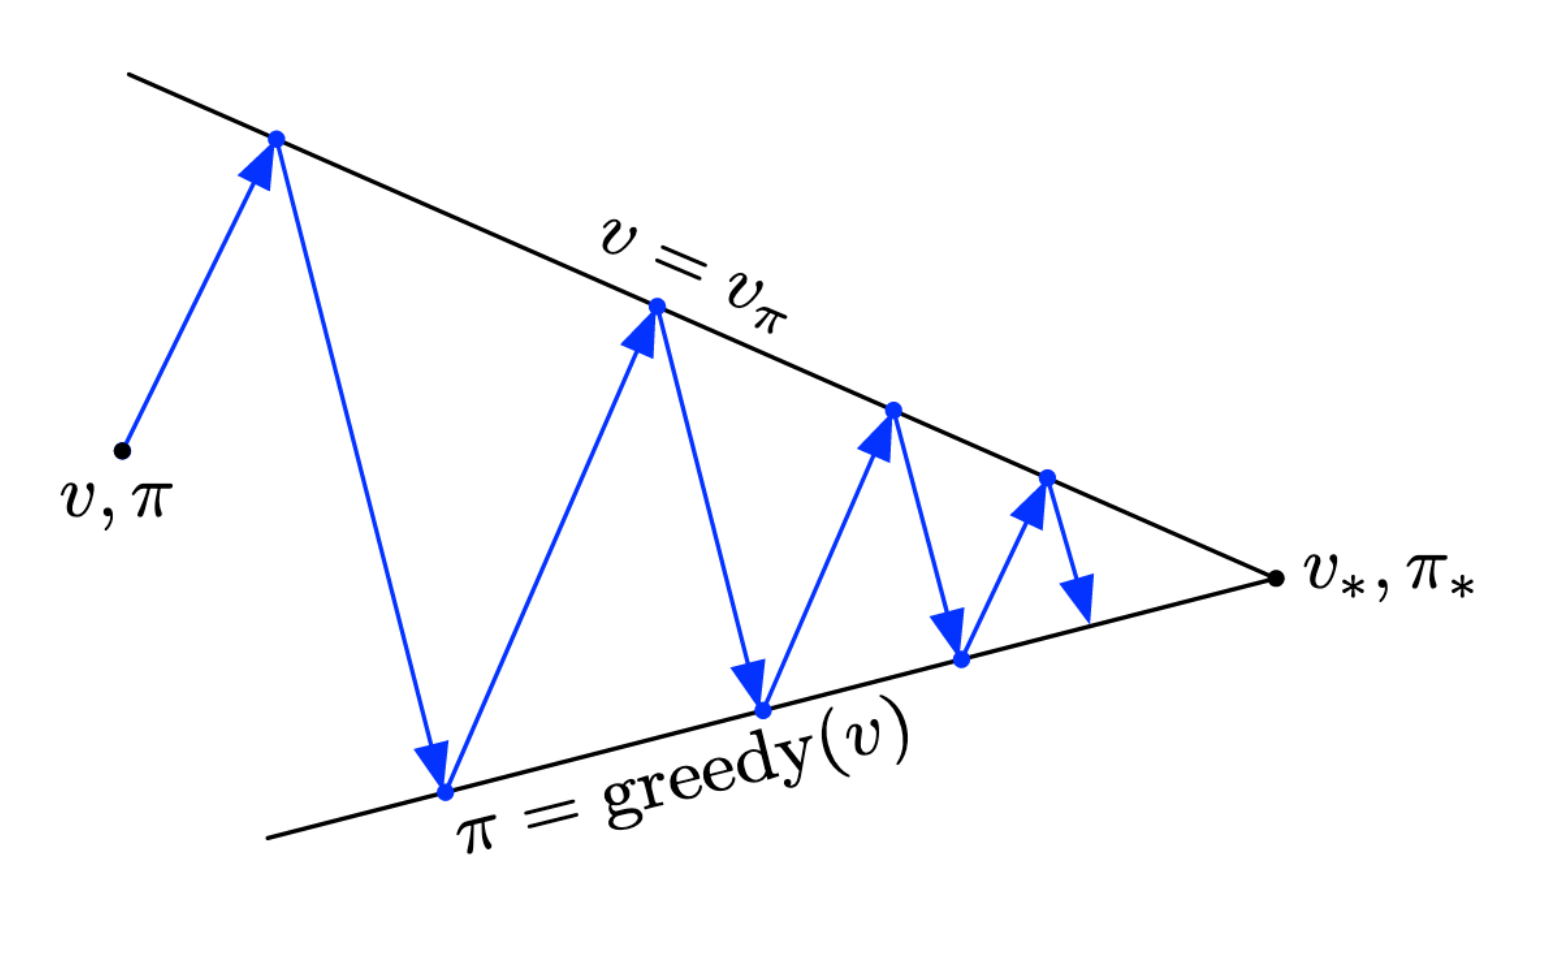
\includegraphics[width=\marginparwidth]{figs/gpi}\\\small Generalised Policy Iteration (GPI)}If \textbf{both the evaluation and improvement stabilise, the value function and policy must be optimal}. The value function stabilises only when it is consisent with the current policy and policy stabilises only when it is greedy with respect to the current value function. Both stabilising implies that a policy has been found which is greedy with respect to its own evaluation function, implying that the Bellman optimality equation holds. 

Whilst not practical for large problems, DP methods are actually quite efficient with (worst-case) complexity $\Omega(\texttt{poly}(n, k))$  where $n, k$ are the number of states and actions respectively. They also seem to typically converge must faster than the worst case. 

\ix{Bootstrapping}DP methods update estimates of the values of states based on estimates of the values of successor states; \textbf{bootstrapping}. 



\end{document}